\documentclass[AMA]{WileyNJD-v1}

\articletype{Article Type}%

%\received{26 April 2016}
%\revised{6 June 2016}
%\accepted{6 June 2016}
%% AMA style

%\usepackage[bibstyle= nature, citestyle=numeric-comp, sorting=none]{biblatex}

%\usepackage[sort,numbers]{natbib}
%

 
%
\bibliographystyle{unsrt}

\usepackage{amsmath,amsfonts,amsxtra,amssymb,latexsym,amscd,amsthm,}
\usepackage{epstopdf} 
\usepackage{tabularx}
\usepackage{graphics}
\usepackage{graphicx}
\usepackage[utf8]{inputenc}
\usepackage[T1]{fontenc}

%\usepackage[bibstyle= nature, citestyle=numeric-comp, sorting=none]{biblatex}

%\raggedbottom

\begin{document}
	
\title{Joint Fast Time Domain Channel Estimation with ICI Cancellation for LTE-R Systems}

\author[1]{Van Duc Nguyen*}
\author[1]{Van Vinh Duong}
\author[2]{Hanbyeog Cho}
\author[3]{Seong-Gyoon Park}
\author[1]{Tien Hoa Nguyen}

\authormark{VAN DUC NGUYEN \textsc{et al}}


\address[1]{\orgdiv{School of Electronics and Telecommunications}, \orgname{Hanoi University of Science and Technology}, \orgaddress{\state{Hanoi}, \country{Vietnam}}}

\address[2]{\orgdiv{Smart Mobility Research Department }, \orgname{ETRI}, \orgaddress{\state{Daejeon}, \country{Korea}}}

\address[3]{\orgdiv{School of Information and Communication}, \orgname{KongJu National University}, \orgaddress{\state{Daejeon}, \country{Korea}}}

\corres{*Van Duc Nguyen, \email{duc.nguyenvan1@hust.edu.vn}}
	
%\presentaddress{This is sample for present address text this is sample for present address text}
	
\abstract[Summary]{The core modulation technique Orthogonal Frequency Division Multiplexing (OFDM) is widely integrated in LTE Communication Platform (LTE-R) that supports for intelligent transportation systems (ITS). In such systems, the large Doppler spread is introduced due to the movement of high-speed railway (HSR). Consequently, the orthogonality of subcarriers is destroyed resulting in the inter-carrier interference (ICI). In addition, the high relative movement speed of the transceivers leads to a very fast-time varying channel, which changes within an OFDM symbol. To track the time variation of the channel, we apply a pilot based channel estimation (CE) technique in time domain using the Cubic Hermite interpolation for OFDM systems. We propose a novel pilot structure for high mobility channel to improve the estimation accuracy of channel impulse response (CIR). We then use the estimated channel to compute the CIR channel matrix to cancelate the ICI in the received signal. To evaluate the performance of the proposed method, the D2a scenario of the WINNER II channel model has been used. Simulation results show that our proposed technique outperforms the state-of-the-art in terms of channel estimation and ICI cancellation performance.}
	
\keywords{LTE-R; HSR; OFDM; ICI Cancellation; Time-varying Channel; Channel Estimation.}	
\jnlcitation{\cname{%
			\author{Van Duc Nguyen}, 
			\author{{Van Vinh Duong}, 
			\author{Hanbyeog Cho}, 
			\author{Seong-Gyoon Park}, and 
			\author{Tien Hoa Nguyen}} (\cyear{2018}), 
		\ctitle{Joint Fast Time Domain Channel Estimation with ICI Cancellation for LTE-R Systems}, \cjournal{International Journal of Communication Systems}, \cvol{201x;00:1--6}.}}
	
\maketitle
	
\footnotetext{\textbf{Abbreviations:} DTTB, Digital Terrestrial Television Broadcasting; ETCS, European Train Control System; UIC, International Union of Railway; ETCS, European Train Control System; CSI, Channel State Information; GI, Guard Interval}
	
	
\section{Introduction}\label{section-1}

The next generation of mobile broadband network standard (Next-G) uses the OFDM technique, which has become a core technology employed by many wireless communication standards such as of LTE, DTTB (Digital Terrestrial Television Broadcasting) and IEEE 802.11 families, etc.. The popularity of OFDM in such the system has been made since it can provide a high data rate transmission and efficiently deal with the multi-path propagation problem. 
	
With the development of the high-speed vehicular communications, Long Term Evolution for Railway (LTE-R) has been already became communication standard in high speed railway (HSR) environment \cite{Luo2012,Fokum2010}, where the transportation speed can be up to 500km/h \cite{Banerjee2016}. A number of standardizations for HSR have been setup, which are known as European Train Control System (ETCS) or International Union of Railway (UIC). The high relative movement of transceiver introduces the  rapidly time-variation of the channels as well as a large Doppler shift. Therefore, the major problem in designing the LTE-R system is to meet the condition of the high-speed movement of the receiver. For instance, the relative mobility of the transceiver at a speed of 500km/h and on a carrier frequency of 2.6GHz, causes the the Doppler shift of 1204Hz. In this transmission scenario, the channels have a coherence time in the order of the symbol period,  thus the channel need to be estimated from OFDM symbol to symbol \cite{Barhumi2005}.

Although many researches have been carried out on channel estimation (CE) for the fast time-varying channels, most of the previous methods was applied under the assumption that the CIR is stationary within an OFDM block \cite {Hu2003, Tang2007, Park2005}. Conventional CE methods use pilot symbols inserted in the transmitted data sequence. The channel state information (CSI) at the positions of the pilot symbols can be obtained by one-tap channel equalizer. The channel coefficients corresponding to the data symbols can be reconstructed by interpolation techniques \cite{Cavers1991, Lau1994}, or by different kinds of filters. Interpolation or filter techniques can be applied in both time and the frequency domain \cite{Mostofi2005,Hijazi2009,Simko2011}. Some of the well-known filters for channel estimation are the  Least Squares (LS), Minimum Mean Square Error (MMSE)  \cite{Mostofi2005,Hijazi2009,Simko2011} and the Kalman filter \cite{Kaufman1983}, whereas the MMSE filter provides a better performance than that obtained by LS \cite{Edfors1998}. The Kalman filter is also a good candidate to track a fast time-varying process, but the Kalman filter has its limitation in tracking a number of channel parameters at a same time \cite{Kaufman1983}. Moreover, these methods need to have sufficient number of inserted pilot symbols to compute the filter coefficients and the channel correlation matrix information must be available at the receiver. This assumption is not always practical and have a high complexity because of the matrix inversion. 

The LTE-R channel suffers from frequency and time-selectivity, which is named as doubly-selective channels \cite{Adireddy2002,Fan2014}. In addition, one of a major characteristic of the LTE-R channels is time-invariant within an OFDM symbol. The channel can be estimated in the time or frequency domain. However, the frequency domain CE could not applied to estimate the fast time-varying channel. This is because the frequency  domain CE must have an assumption that the channel does not change within an OFDM symbol. If this condition is not maintained, the estimated channel does not reflect to the real channel. Thus, our motivation is to propose a time domain channel estimation method. Afterwards, the estimated CSI will be used to compute the ICI matrix in order to cancelate the ICI components. In the proposed time domain CE method, a novel pilot structure has been deployed, whereas the so-called zero guard interval (GI) is used to protect the pilot symbol from the multi-path interference. A zero signal sequence with the same length of the GI is inserted next to the pilot symbol. This zero signal is the reserved place  to obtain CIR from the received pilot symbols. In context of LTE-R, the CIR changes rapidly, thus it requires an effective interpolation technique to reconstruct the CSI in an OFDM symbol. Instead of using the conventional method such as MMSE or LS filter, we propose to use the Cubic Hermite interpolation method to obtain the CIR information at the data symbol's position.

The Cubic Hermite interpolation technique  uses the first derivative CIR at  the positions of the pilot symbols to calculate the coefficients of the polynomial interpolation function. As a result, the complexity of channel estimation is significantly reduced in comparison to the frequency domain pilot-based CE. 

	
The rest of this paper is organised as follows. In Section \ref{section-2}, we briefly describes the channel model and the OFDM system model designed for the HSR environment. Section \ref{section-3} outlines the proposed CE method based on Cubic Hermite interpolation. Simulation results are discussed in Section \ref{section-4}. Section \ref{section-5} concludes the paper.
	
	
\section{Description of OFDM System using a Time-Domain Pilot Structure for CE}\label{section-2}
	
\subsection{Fast Time-Varying Channel modelling}\label{section-2.1}

With regards to an investigation of channel estimation techniques for LTE-R systems, a realistic HSR transmission multi-path propagation channel is modelled by the the Monte Carlo method. The D2a scenario of the WINNER II channel is adopted as the typical HSR multi-path fading propagation \cite{Guan2011}. A mathematical description of frequency-selective and time-variant channel is given in \cite{Matz2011}, which can be defined as follows
%
\begin{equation}\label{eq:math channel}
	h(\tau,t)=\sum_{l=0}^{N_p-1}h_l e^{j(2\pi f_{D_l}(t)t+\theta_{l})\sigma (\tau-t)},
\end{equation}
%
where the $N_{p}$ is number of channel path, and $h_{l}$ is the amplitude of path $l$th. The function $f_{D_l}(t)$ and $\theta_{l}$ denote the Doppler frequency of path $l$th observed at the absolute time $t$ and the Doppler phase of path $l$th. The popular Monte Carlo channel modeling method, which has been presented in \cite{Nguyen2004}, is used in this paper for the purpose of channel modeling. For implementing the Monte Carlo method, the CIR in Equation (\ref{eq:math channel}) can be rewritten as
%
\begin{equation}\label{eq-math Monte channel}
	h(\tau,t)=\frac{1}{\sqrt{M}}\sum_{l=0}^{N_p-1}h_{l}\sum_{q=1}^{M}e^{j(2\pi f_{l,q}t+\theta_{l})}\delta(\tau-\tau_{l}),
\end{equation}
%
where $f_{l,q} = f_{D_{max}} \text{sin}(2\pi u_{l,q})$, $\theta_{l,q} = 2\pi u_{l,q}$ and $M$ are Doppler frequency, Doppler phase, and number of harmonic function, respectively. Let $u_{l,q}$ denote random variable in range [0,1] with uniform distribution. 
	
We assume that the channel in HSR environment can be characterized by its power delay profile (PDP) and Doppler spectrum. Figure \ref{fig:rhod2achannel} illustrates the modeled channel  with the parameters taken from \cite{Guan2011}, with the bandwidth $B=10$MHz and sampling period $t_a=\dfrac{1}{B}=100$ns. But since the PDP was not coincide with the sampling rate in our simulated system, we interpolated the PDP to fit with the sampling period, and this result will be used for simulation in the end of this paper.
%
\begin{figure}
		\centering
		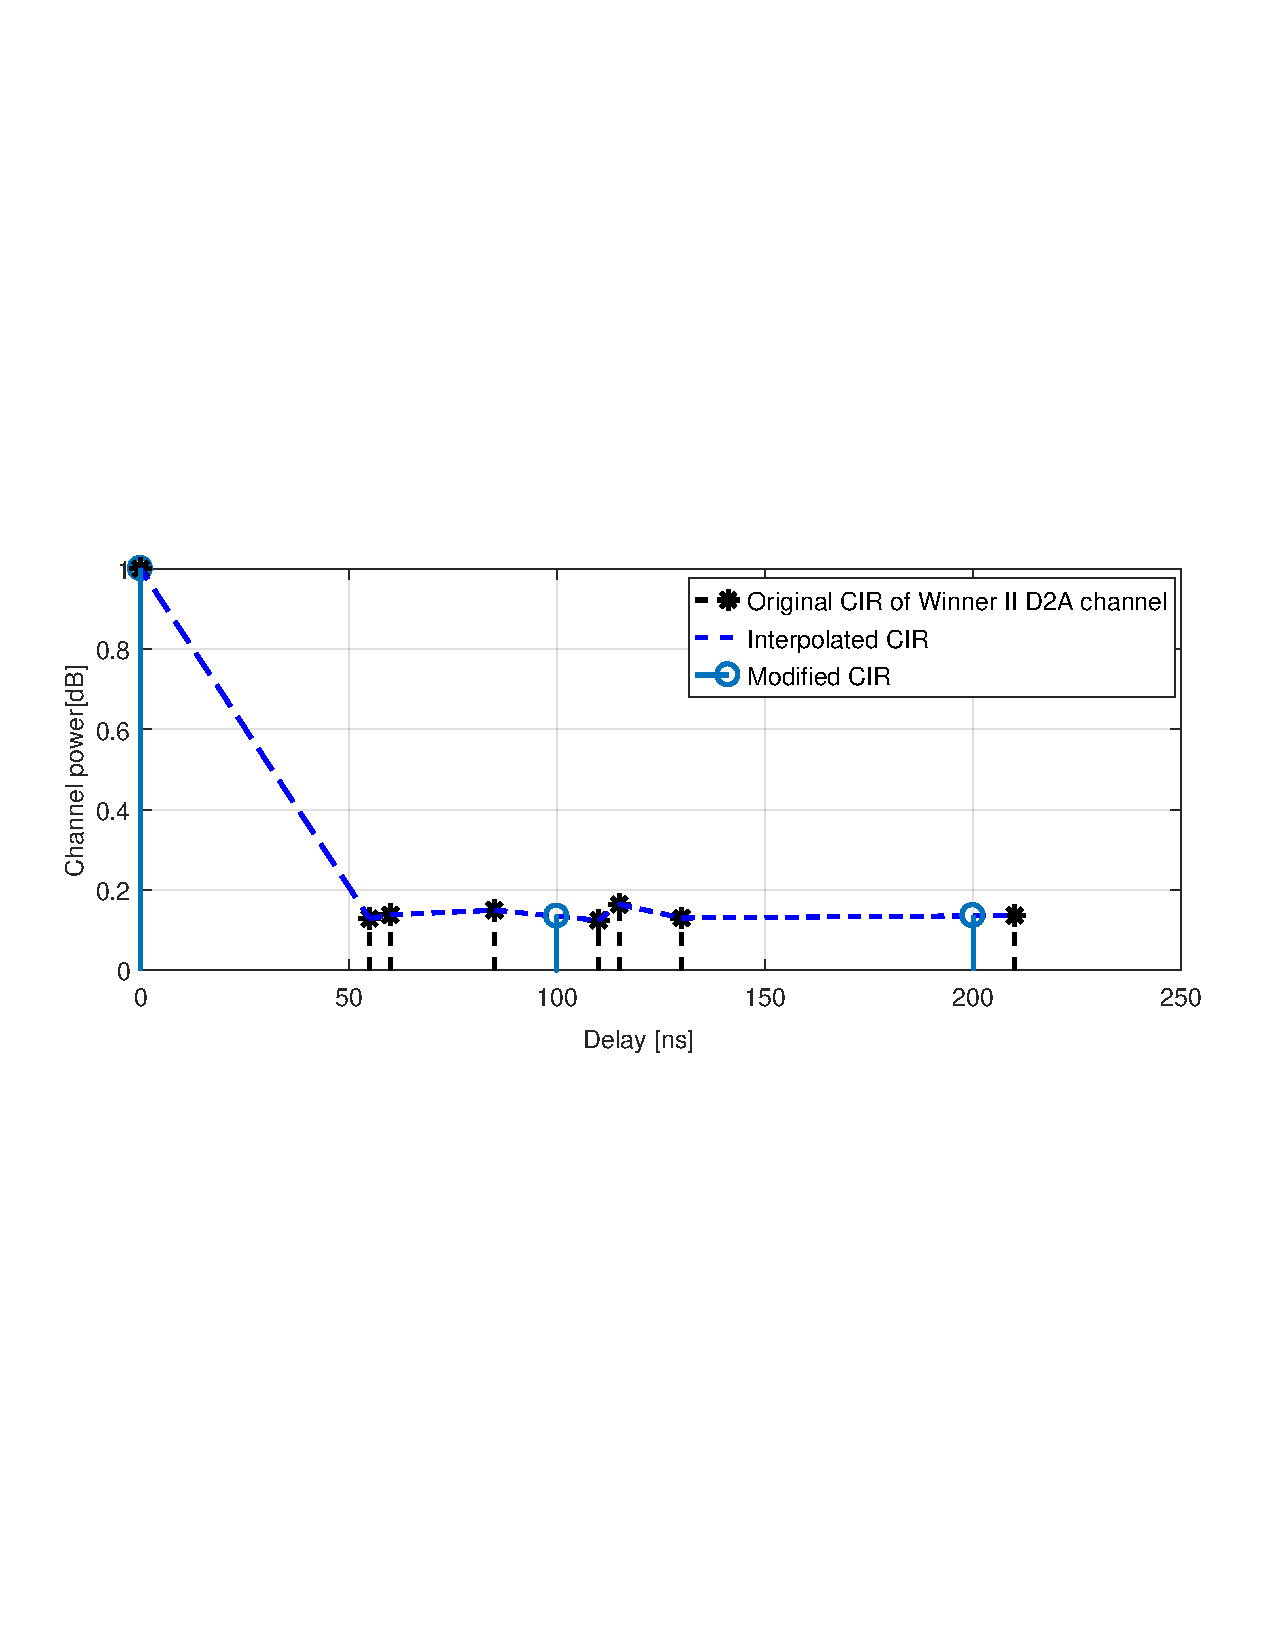
\includegraphics[width=1.0\linewidth]{figures/ChannelPowerModified.pdf}
		\caption{PDP of the simulated channel modified from the WINNER II D2A channel}
		\label{fig:rhod2achannel}
\end{figure}
	
\subsection{OFDM System using a Time-Domain Pilot Structure}\label{section-2.2}
	
We consider the LTE-R system, which is based on the OFDM technique. We denote $N_{c}$ as the number of subcarriers, and $B$ as the system bandwidth. According to the Nyquist theory, the sampling period is obtained by $t_{\rm a}=1/B$. Let $X^{(i)}_{k}= [X^{(i)}_{0} X^{(i)}_{1} \dots  X^{(i)}_{N_c-1}]^{T}$ denote the transmitted signal of $k$th sub-carrier, and at the $i$th OFDM symbol. After using Inverse Fast Fourier Transform (IFFT) to convert $X^{(i)}_{k}$ to the time domain, the transmitted signal is mapped to a novel pilot symbol structure as depicted in Figure \ref{fig:pilot-pattern}. The pilot symbol structure consists of  $2N_G+1$ samples with all zero samples except the middle position, i. e. $p^{(i)}=[0_{1\times N_G}\quad P\quad  0_{1\times N_G}]$, where $N_G$ is the guard interval length. The first  $N_G$ symbols playes the role of the zero guard interval, whereas the second half $N_G$ symbol are reserved to receive the multi-path components of the CIR. To avoid the intersymbol interference (ISI), $N_G$ must be larger than the CIR length $N_p$. The OFDM symbol in the time domain is represented by the  vector $x^{(i)}=[0_{1\times G}\quad P\quad  0_{1\times G}\quad  x^{(i)}_{0} x^{(i)}_{1} \dots x^{(i)}_{N_c-1}]^{T}$ with the length of $ N_{sym}=N_c+2N_G+1$.
%
\begin{figure*}[t]
		\centering
		\includegraphics[width=0.9\linewidth]{"figures/pilot pattern"}
		\caption{The novel pilot structure for channel estimation in HSR environment }
		\label{fig:pilot-pattern}
\end{figure*}
%	
	
After traveling through the multi-path transmission environment, the received signal $ y^{(i)}(n)$ observed at the $i$-th OFDM symbol and the $n$-th sampling interval can be written as
%
\begin{equation}\label{eq-time received signal} 
	y^{(i)}(n)= \sum_{l=0}^{{N_p}-1}h^{(i)}(l,n) x^{(i)}(n-l) + w^{(i)}(n),
\end{equation}
%
where $h^{(i)}(l,n)$  and  $w^{(i)}(n)$ denote the CIR coefficient associated with the $i$th OFDM symbol, and the $l$-th multi-path reflection, and  the additive white Gaussian noise (AWGN) at the  $n$-the sampling interval, and the $i$th OFDM symbol, respectively.
	
After removing pilot symbols, the frequency domain received signal is obtained after taking the FFT of $y^{(i)}(n)$ as follows:
%
\begin{equation}\label{eq:freq-received-signal}
	\begin{split}
	Y^{(i)}(k)&=\dfrac{1}{N} \sum_{n=0}^{N-1} y^{(i)}(n)e^{-j2\pi kn/N}\qquad\\
	&= \sum_{m=0}^{N-1}\sum_{l=0}^{N_p-1} X^{(i)}(m)H^{(i)}_{l}(m-k) e^{-j2\pi lm/N}  \\
	& + W^{(i)}(k), \hspace{0.3cm}k=0,\dots,N-1,
	\end{split}
\end{equation} 
%
where $W^{(i)}(k)$ and $H^{(i)}_l(k)$ denote the Fourier transform of $w^{(i)}(m)$ and $h^{(i)}(l,n)$, respectively. $H^{(i)}_{l}(k)$ is defined as
%
\begin{equation}\label{eq:fft-of-CIR}
	H^{(i)}_{l}(k)=\frac{1}{N} \sum_{n=0}^{N-1} h^{(i)}(l,n)e^{-j2\pi nk/N}.
\end{equation}
%
The received signal in \eqref{eq:freq-received-signal} can be formulated in the vector form as follows:
%
\begin{equation}\label{eq:vector-sinal}
	\rm {\textbf Y^{(i)}}= \rm{\textbf H^{(i)} X^{(i)}} +\rm {\textbf W^{(i)}}, 
\end{equation}
%
where ${\rm{\textbf Y^{(i)}}}=[Y(0),Y(1), \dots,Y(N-1)]^{T}$,  ${\rm {\textbf X^{(i)}}} =[X(0), X(1), \dots,X(N-1)]^{T}$ and  ${\rm {\textbf W^{(i)}}}=[W(0),W(1), \dots, W(N-1)]^{T}$, are the vectors of received, transmitted signal, and the Gaussian noise components, respectively. The channel matrix $\rm{\textbf H^{(i)}}$ is defined by
%
\begin{equation}\label{eq:matrix-channel}
	\rm{\textbf H^{(i)}}=\left[\begin{array}{cccc}
	a_{0,0}& a_{0,1} &  \cdots &  a_{0,N-1} \\
	a_{1,0}&  a_{1,1}&  \cdots &  a_{1,N-1}  \\
	\vdots &  \ddots&  \vdots \\
	a_{N-1,0}&  a_{N-1,1}&  \cdots &  a_{N-1,N-1}
	\end{array}\right],
\end{equation}
%
with elements $a_{m,k}$ can be obtained as 
%
\begin{equation*}
a_{m,k}=\sum_{l=0}^{N_p-1}H^{(i)}_l(k-m) e^{-j2\pi ml/N},m,k=0,1,\dots,N-1.
\end{equation*}
%
	
If the CIR is time-invariant withing an OFDM symbol period, then the off-diagonal elements $a_{m,k}$ $(k\neq m)$ of matrix $\rm{\textbf H^{(i)}}$ are approximately equal to zero. In this case, ICI components does not exist, and thus, the orthogonality of the transmitted signal will be preserved. As the result, the signal at receiver can be detected by computing the channel matrix inversion as follows:
%
\begin{equation}\label{eq:matrix-inverse}
\rm {\textbf X^{(i)}}= \rm {\textbf H^{(i)}}^{-1}{\rm {\textbf Y^{(i)}}}.
\end{equation}
%
	
However, in LTE-R case, the channel cannot be considered as time  unchanged during an OFDM period, the rapidly time-varying of channel and large Doppler spread destroy the orthogonality between subcarriers. Therefore, the matrix $\rm{\textbf H^{(i)}}$ is not the diagonal matrix, and the off-diagonal elements introduce ICI. Solving  the equation \eqref{eq:matrix-inverse} by matrix inversion is problematic, especially if its size becomes large. Due to the limit of maximum Doppler shift, only few off-diagonal elements near the main diagonal elements have value lager than zero \cite{Jeon1999}. This leads to the matrix $\rm{\textbf H^{(i)}}$ becoming a banded matrix \cite{Cai2003}. To reduce the complexity of the matrix inversion, we force $a_{m,k}$ to be zeros at the positions far from the diagonal elements of the matrix $\rm{\textbf H^{(i)}}$. Thus,  $a_{m,k}$ in the Eq. \eqref{eq:matrix-channel} can be defined as
%
\begin{equation}
a_{m,k}=0\quad  \text{with}\quad  |k-m|\geqslant q/2,
\end{equation}
%
\begin{figure*}
\begin{equation}\label{eq:banded matrix}
\begin{aligned}
		\rm {\textbf H^{(i)}} = \begin{bmatrix} 
		a_{0,0} & a_{0,1}& \cdots & a_{0,q/2} & 0 & 0 &0
		\\ a_{1,0} & a_{1,1} & \cdots & \cdots &\cdots& 0 & \vdots
		\\ \vdots & \vdots & \ddots & \ddots &\ddots & \ddots &0
		\\ a_{q/2,0} & \cdot & \cdots & \ddots & \ddots & \ddots & a_{N - 1 - q/2,N - 1}
		\\0&\cdot& \cdot& \cdots &\ddots& \ddots &\vdots
		\\ \vdots & \vdots & \ddots & \ddots & \vdots & a_{N - 2,N - 2}  & a_{N - 2,N - 1}
		\\0 &0&0 & a_{N - 1,N -1- q/2}& \cdots & a_{N - 1,N - 2}&a_{N - 1,N - 1}\end{bmatrix}.
	\end{aligned}
	\end{equation}
\end{figure*}
where $q$ is the size of the band matrix, which indicates the number of dominant ICI terms. The matrix $\rm{\textbf H^{(i)}}$ can be rewritten as expressed in (\ref{eq:banded matrix}).
	
One of the main complexity sources of equalization is inverse of matrix, which can be reduced by exploiting  the banded structure of $\rm{\textbf H^{(i)}}$. A large number of works have been done to solve this problems in \cite{Hsu2009, Liu2012, Schniter2004, Fang2007}. However, in order to construct the channel matrix in \eqref{eq:matrix-channel}, it is compulsory to have complete knowledge of the CIR, $h^{(i)}(l,n)$ in each OFDM symbol. In the HSR environment, the channel varies even within an OFDM symbol so that it is very challenging to estimate the channel, as well es to perform the ICI equalizer in the real time signal processing condition. Hence in the next sections, we propose receiver architecture, which joins the  time domain channel estimation with ICI cancellation for LTE-R system over a very fast time-varying channel.
	
\section{Interpolation techniques for time domain channel estimator}\label{section-3}
	
In this section, we describe some conventional interpolation techniques, and propose our interpolation scheme for channel estimation in the time domain. One of criteria to measure the time-variation of the channel is the normalized Doppler frequency shift, $\varepsilon = T_{sym}\times f_{d}$, where $f_{d}$ and $T_{s}=N_{sym}\times t_{a}$ are the Doppler frequency and the duration of one OFDM symbol, respectively. Table \ref{ta:Normalize-frequency-offset} shows the value of normalized Doppler frequency shift, $\varepsilon$, in dependence of the movement speed of the receiver. The corresponding CIRs are plotted in Figure \ref{fig:cir-variation}, to demonstrate the time-variation of the channel. It can be seen that at the movement speed below 200 km/h, the channel varies nearly as a linear function  within an OFDM duration. However,  if the normalized Doppler frequency shift, $\varepsilon$, is above 0.075, which corresponds to the movement speed of 300 km/h on a frequency of 2.6GHz, then the channel does not follow a linear fashion. In such situation, the linear interpolation within an OFDM symbol does not provide a good system performance.
	
To obtain the good channel estimation in the condition of the time-variation within an OFDM symbol as depicted in Figure \ref{fig:cir-variation}, we propose a channel estimation method using the pilot symbol structure described in Figure \ref{fig:pilot-pattern}, where the first $N_G$ zero symbols are used for the guard interval, following is the pilot symbol, and the next $N_G$ zero symbols are reserved to receive the multipath components of the CIR. The  first $N_G$ zero symbols are the guard interval for protecting the system from ISI, while the second  $N_G$ zero symbols is to protect the received pilot symbols from the overlapping with the data symbols. We call these  $N_G$ zero symbols as {\it{"the pilot guard interval"}}. If the guard interval lenght is selected to be larger than the maximal time delay of the channel, i.e. $T_{G} \geqslant \tau_{max}$ (${T_{G}=N_G \times t_a }$), then all received pilot symbols within an OFDM symbols should be located in the areas of the pilot guard interval.


We observe the received pilot symbol at the sampling index $n_p$, whereby $G\leq n_p \leq G + l$ $l$ is the multi-path index, which follows the condition $0\leq l \leq N_p $.  At the $i$th transmitted OFDM symbol, the received pilot symbol corresponding to the $l$ path can be written as:
	%
	\begin{equation}\label{eq:received-pilot-symbol}
	y^{(i)}_{p}(n_p) = \sum_{l = 0}^{N_p - 1} h^{(i)}_{p}(l,n_p) \times P  + w^{(i)}_{p}(n_p),                 
	\end{equation}
	%	
where $P$ is the complex value of the transmitted pilot symbol, and $w^{(i)}_{p}(n_p)$ is the additive noise added to the received pilot symbol. As depicted in Figure \ref{fig:pilot-pattern}, the pilot symbols are transmitted repeatedly with a period of an OFDM symbol. The information of a channel reflection path is periodically obtained from the received pilot symbols. As shown in Figure  \ref{fig:cir-variation}, the channel coefficients  of each channel reflection path vary with an OFDM symbol. Thus, interpolation techniques need to be deployed to recover the channel information between the gap of two consecutive received pilot symbols relating a channel multipath reflection. 

\subsection{Linear Interpolation technique}
It is clear that from (\ref{eq:received-pilot-symbol}) the CIR coefficient corresponding the $l$ reflection path, and at the $i$-th OFDM symbol, and  at $n_p$ sampling index  can be obtained by
%
\begin{equation}\label{eq:CIR-at-pilot}
	h^{(i)}_{p}(l,n_p)= \dfrac{y^{(i)}_{p}(n_p)}{P}.
\end{equation}
%
The linear interpolation technique used for time domain channel estimation is described in \cite{Jeon1999}. The advantage of this method is low complexity, however, it provides the poor performance, especially at high movement speed of the receiver, namely from 300-500km/h. To improve the channel estimation performance, we propose a Cubic Hermite interpolation method described in the next sub-section.
%
	\begin{figure}
		\centering
		\includegraphics[width=1.0\linewidth]{"figures/CIR_variation_speed"}
		\caption{Amplitude variation of CIR  in time domain}
		\label{fig:cir-variation}
	\end{figure}
	
	
\subsection{Proposal of using the Cubic Hermite Interpolation for time domain CE}
	
The time domain  channel estimation scheme  is conducted in the three steps as follows:
	
\rm{\textbf {Step 1:} The channel coefficients of each channel tap at the pilot guard interval positions are estimated by using the Equation (\ref{eq:CIR-at-pilot}). Afterwards, the channel coefficients at data positions are obtained by using the Cubic Hermite interpolation. 
		
		
\rm{\textbf {Step 2:} Based on the estimated CIRs at the positions of the pilot guard interval of the two consecutive OFDM symbols, namely $h^{(i)}_{p}(l,n_p)$ and $h^{(i+1)}_{p}(l,n_p)$,  the CIRs at the data position $\tilde h^{(i)}(l,n)$  can be obtained  by using the Cubic Hermite function, which can be written as 
%
\begin{equation}\label{eq:cubic-hermite}
			\tilde h^{(i)}(l,n) = C_3(n - n_{p})^3 + C_2(n - n_{p})^2 + C_1(n-n_{p}) + C_0,
\end{equation}
%
where $i\times T_{s}\leq n\leq (i+1)\times T_{s}$. The coefficients of the Cubic Hermite function can be defined as
\begin{align*}
			\centering
			C_3 &= \frac{d^{(i)}_{l}+d^{(i+1)}_{l}-2{\Delta {\delta _i}}}{(\lambda_{i})^2},\\
			C_2 &= \dfrac{-2d^{(i)}_{l}-d^{(i+1)}_{l}+3{\Delta {\delta _i}}}{\lambda_{i}},\\
			\qquad C_1 &=d^{(i)}_{l},\\
			C_0 &= h^{(i)}_{p}(l,n_p).
\end{align*}	
%
			
Here, $d^{(i)}_{l}$ and $d^{(i+1)}_{l}$ represent the first derivative of the CIR function of the $l$th channel path,  at the pilot symbol positions embedded in the  $i$-th and $(i+1)$-th, OFDM symbol, respectively. The interval ${\lambda_{i}} = {n_p}^{i+1}-{n_p}^{i} $ denotes the distance between two consecutive received pilot symbols, which are associated with the  $l$-th channel path. The coefficient ${\Delta {\delta _i}}$ is calculated by
%
\begin{equation*}
	\centering
	\Delta {\delta _i} =\frac{h^{(i+1)}_{p}(l,n_p) - h^{(i)}_{p}(l,n_p)}{\lambda_{i}}.
\end{equation*}
%
\begin{figure}
		\centering
		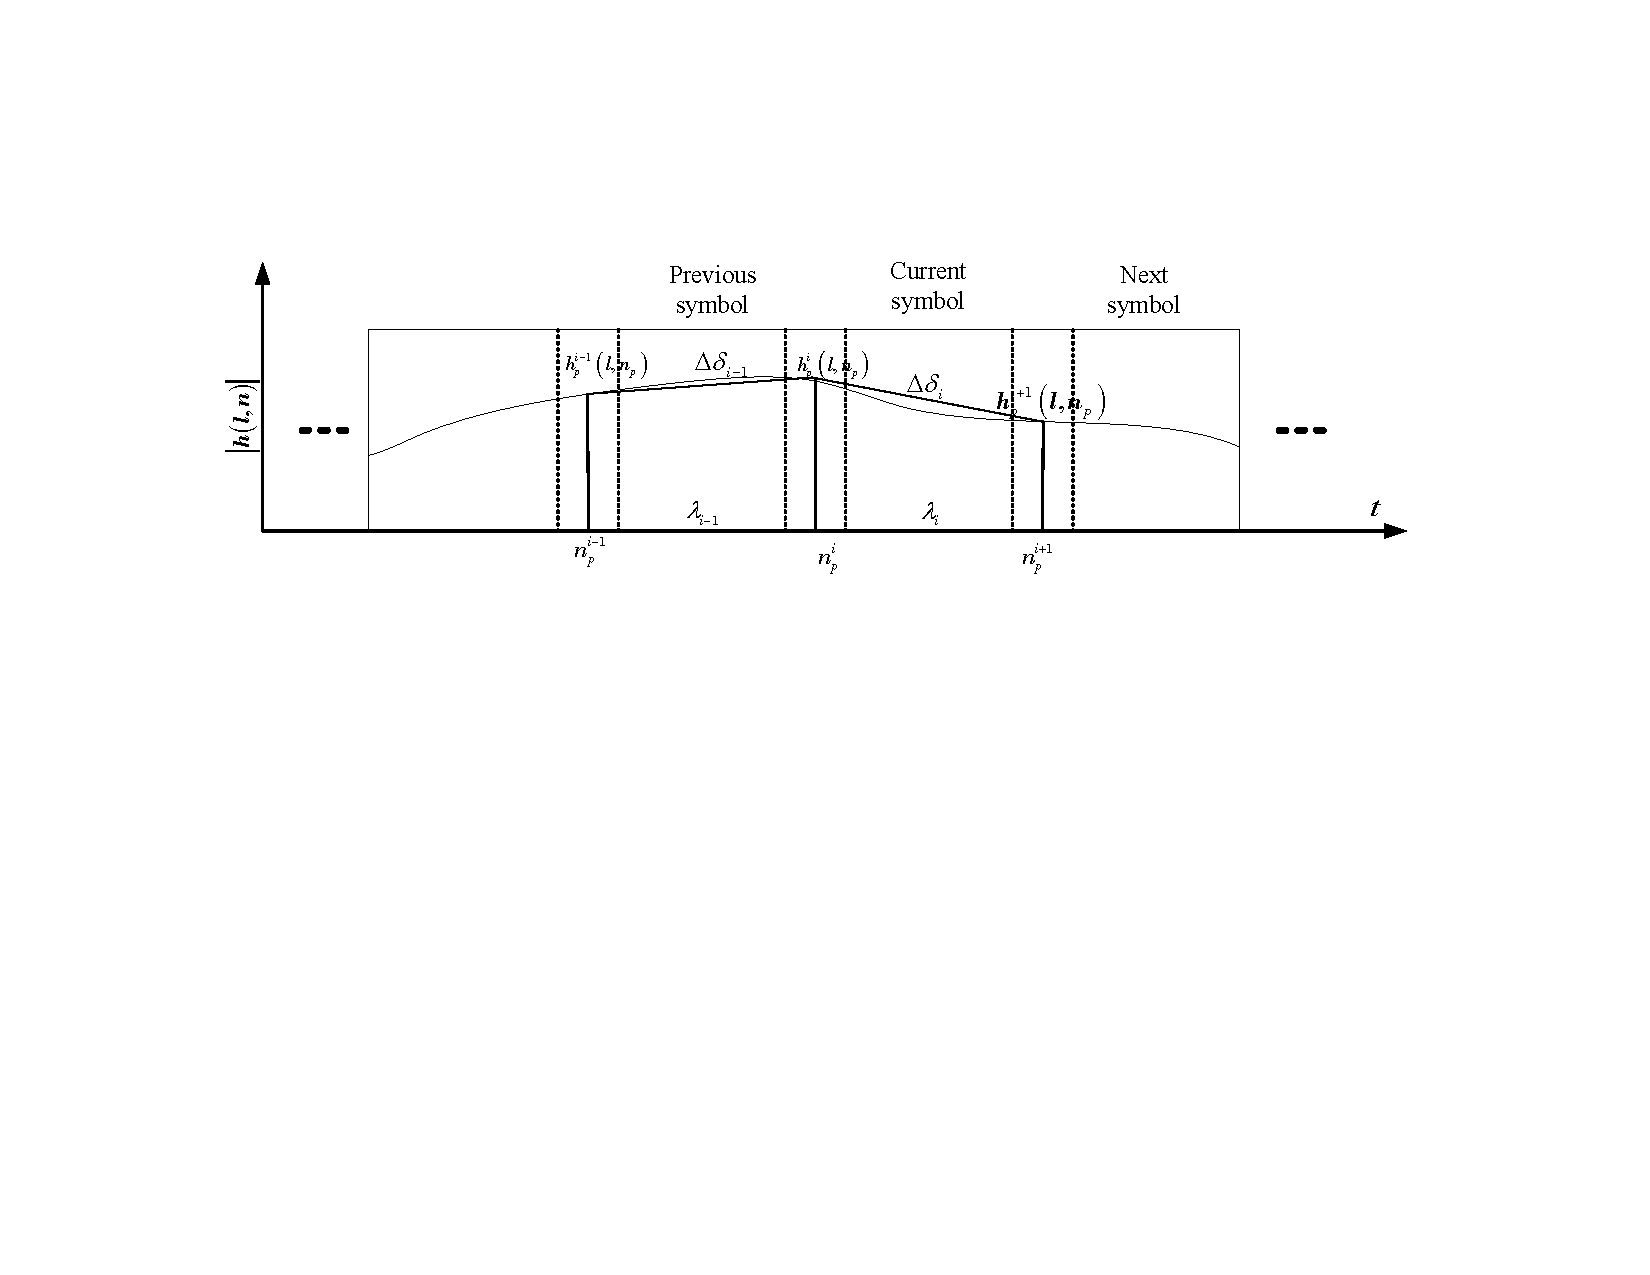
\includegraphics[width=1.0\linewidth]{figures/derivative_cubic_hermite}
		\caption{Cubic Hermite interpolation in three consecutive OFDM symbols}
		\label{fig:derivativecubichermite}
\end{figure}	
%			
Compare to the cubic spline interpolation technique, the Cubic Hermite interpolation method has lower complexity. This is because the earlier one requires the second derivative of the CIR functions, while the later one needs only the first derivative degree. 
In the literature, there are several algorithms to obtain the first derivative $d^{(i)}_{l}$ and $d^{(i+1)}_{l}$, such as  Akima method, Ellis-Mclain method. For the sake of simplicity, we use the method proposed in \cite{ Fritsch1980} to calculate $d^{(i)}_{l}$ as follow
%
\begin{equation}
d^{(i)}_{l} = \dfrac{\lambda_{i}}{\lambda_{i-1}+\lambda_{i}}{\Delta {\delta _{i-1}}} + \dfrac{\lambda_{i-1}}{\lambda_{i-1}+\lambda_{i}}{\Delta {\delta _i}}, 	
\end{equation}
where $i$ is the  OFDM symbol index. For the first and the last OFDM symbol, we set $d^{(i)}_{l}$ to be zero. Figure \ref{fig:derivativecubichermite} illustrates the curve of the  channel coefficient of the $l$ reflection path, which is reconstructed by the Cubic Hermite method over three consecutive OFDM symbols.

			
\rm{\textbf {Step 3:} After performing the Step 1 and 2, the channel matrix in time domain given in (\ref{eq:channel matrix time domain}) with the dimension of $L \times N$ is obtained. The frequency domain channel matrix $\rm{\textbf H^{(i)}}$ is the FFT of CIR matrix  $\rm{\textbf h^{(i)}_{c}}$. Based on the frequency domain channel matrix $\rm{\textbf H^{(i)}}$ , we apply the ICI canceller proposed in \cite{Qiu2010} to cancel the ICI components in the received data. Thus, the system performance will be increased.
%
\begin{equation}\label{eq:channel matrix time domain}
	{
		\rm{\textbf h^{(i)}_{c}}=\left[\begin{array}{cccc}
		{\tilde{h}_{0,0}}& \tilde{h}_{0,1} &  \cdots &  \tilde{h}_{0,N-1} \\
		\tilde{h}_{1,0}&  \tilde{h}_{1,1}&  \cdots &  \tilde{h}_{1,N-1} \\
			\vdots &  \ddots&  \vdots \\
		\tilde{h}_{L-1,0}&  \tilde{h}_{L-1,1}&  \cdots &  \tilde{h}_{L-1,N-1}
		\end{array}\right]}
\end{equation}
%
				
\section{Simulation Results and Discussion}\label{section-4}
	%
	\begin{table}
		\centering
		\caption{Channel and system parameters for simulations}
		\label{ta:parameters}
					\begin{center}
						\begin{tabular}{|l|r|}
							\hline 	
							Parameters & Values\\
							\hline 
							Carrier Frequency(GHz)  &  2.6   \\
							\hline
							System Bandwidth(MHz) & 10\\
							\hline
							Number of FFT & 1024\\
							\hline
							Channel Type & Winner II (D2a)\\
							\hline
							Modulation Mode & 16QAM\\	
							\hline
							
		\end{tabular}
	\end{center}
\end{table}
				
				
\begin{table}
		\centering
		\caption{The normalized Doppler frequency offsets}
		\label{ta:Normalize-frequency-offset}
		\begin{center}
			\begin{tabular}{|l|r|r|r|r|r|r|}
				\hline 	
				Velocity(km/h) & 100 & 200 & 300 & 400 & 500  \\
				\hline 
			{$\varepsilon=f_{d} \cdot T_{s} $} & 0.025 &0.05 & 0.075 & 0.1 & 0.125 \\
				\hline 
			\end{tabular}
		\end{center}
\end{table}
				
To demonstrate the performance of the proposed time domain channel estimation method, we simulate an OFDM system using the LTE-R paramters as given in Table \ref{ta:parameters}. The  WINNER II D2a channel  is modelled by the Monte Carlo simulation method described in the subsection \ref{section-2.1}. The carrier frequency $f_c$ is selected to bo 2.6 GHz.

%In this section, to demonstrate the effectiveness of our proposed CE method for fast %time-variant multi-path channel, we compare the performance of our system with conventional CE %frequency domain and Jeon's CE time domain schemes by Monte Carlo simulation. The OFDM system %parameters used in the simulation are illustrated in Table \ref{ta:parameters}. The mean %squared error (MSE) and the symbol error rate (SER) performances are examined in terms of the %average signal-to noise (SNR) ratios and maximum Doppler spread $(f_{d}T_{s})$ for the Winner %II D2a channel model. 
				
Figure \ref{fig:cir722hz} shows  the  CIR estimated by the proposed method at a SNR of  30dB, and for a Doppler frequency  $f_{d}$ of 722Hz. At the carrier frequency of 2.6 GHz, this Doppler frequency corresponds to a train speed of 300km/h. The channel estimation performance obtained by the Jeon's method using the linear interpolation technique described in \cite{Jeon1999} is provided for comparison purpose. It can be observed that our proposed estimator fits well with the real channel, and even better than that obtained by the  Jeon's method. 


Figure \ref{fig:1204hz} illustrates the time and frequency domain channel estimation performance in terms of mean square error (MSE) versus SNR. The MSE is calculated by
%
\begin{equation}\label{eq:mse-calculate}
MSE=\dfrac{\sum_{l=0}^{N_p-1}\sum_{n=0}^{N-1} {\mid h_{l,n} - \tilde{h}_{l,n}\mid}^{2} }{{\sum_{l=0}^{N_p-1}\sum_{n=0}^{N-1} {\mid h_{l,n}\mid}^{2}}}
\end{equation}
%
The maximum Doppler frequency $f_{d}$ is of 1204 Hz, which corresponds to a relative speed between transceivers of 500km/h. It can be seen that frequency domain CE does not give a good performance in comparison with that provided by the time domain CE. This is because, if we transfers the received signal to the frequency domain and perform the interpolation, then the interpolation resolution in the time domain is larger than duration of a FFT window, i. e. an OFDM symbol. This introduces the interpolation error, and thus the frequency domain CE is not suitable for very fast time-varying channels. The Jeon's method in \cite{Jeon1999} performs the CE in the time domain, however, liner interpolation is deployed. In addition, the pilot symbol is not well protected as in our proposal by using the so-called zero guard interval. De deployment of the proposed pilot symbol structure and the Cubic Hermite in the time domain for CE shows the better system performance than that obtained by Jeon's method.  
%
\begin{figure}
	\centering
	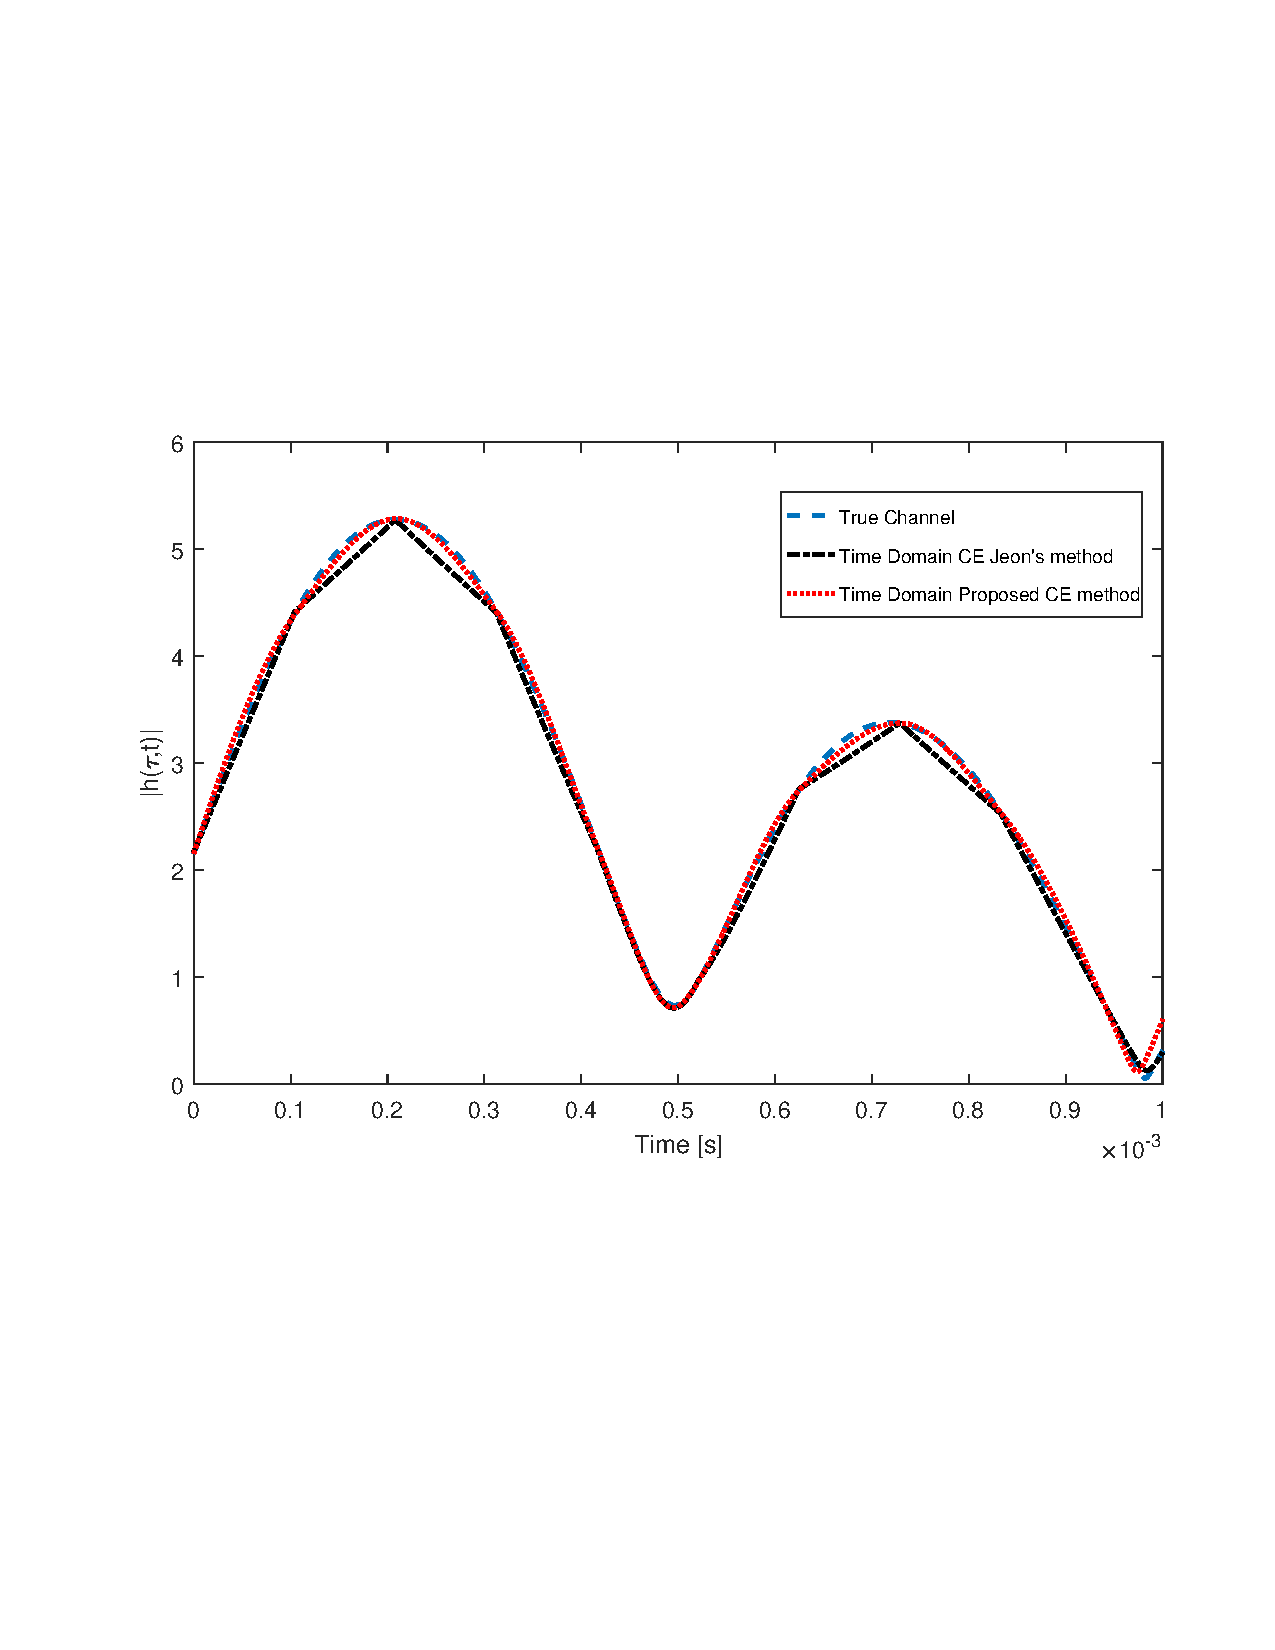
\includegraphics[width=1.0\linewidth]{figures/compare_linear_cubic_org.pdf}
	\caption{Comparison of the amplitude of estimated channel with that of true channel for a Doppler frequency of $f_{d}=722$Hz}
	\label{fig:cir722hz}
\end{figure}
%		
Figure \ref{fig:msespeed} shows the simulation results in terms of the MSE versus the normalized Doppler frequency offsets as given in Table \ref{ta:Normalize-frequency-offset}. In these simulations, the SNR is set to be 30dB. Similar to the results depicted in Figure \ref{fig:1204hz}, our proposed method provides the best system performance. Moreover, it tracks the channel well for a very high Doppler frequency.
				
Figure \ref{fig:ser722hz} shows the system performance in terms of the SER, which are obtained by different CE schemes in combination with the interference cancellation. It is clear, that the CE in frequecy domain provides the lowest system performence. In contrast, the time domain CE schemes including Jeon's and our proposed method yields significant better system performance. 
Compare to the Jeon's method, about  5-7dB of SNR can be gained by using our method to obtain a SER of  $2\times 10^{-2}$  This is because, the accuracy of the channel matrix  $\rm{\textbf H^{(i)}}$ has been improved, and thus the ICI canceller performance becomes better. 
%				
\begin{figure}
	\centering
	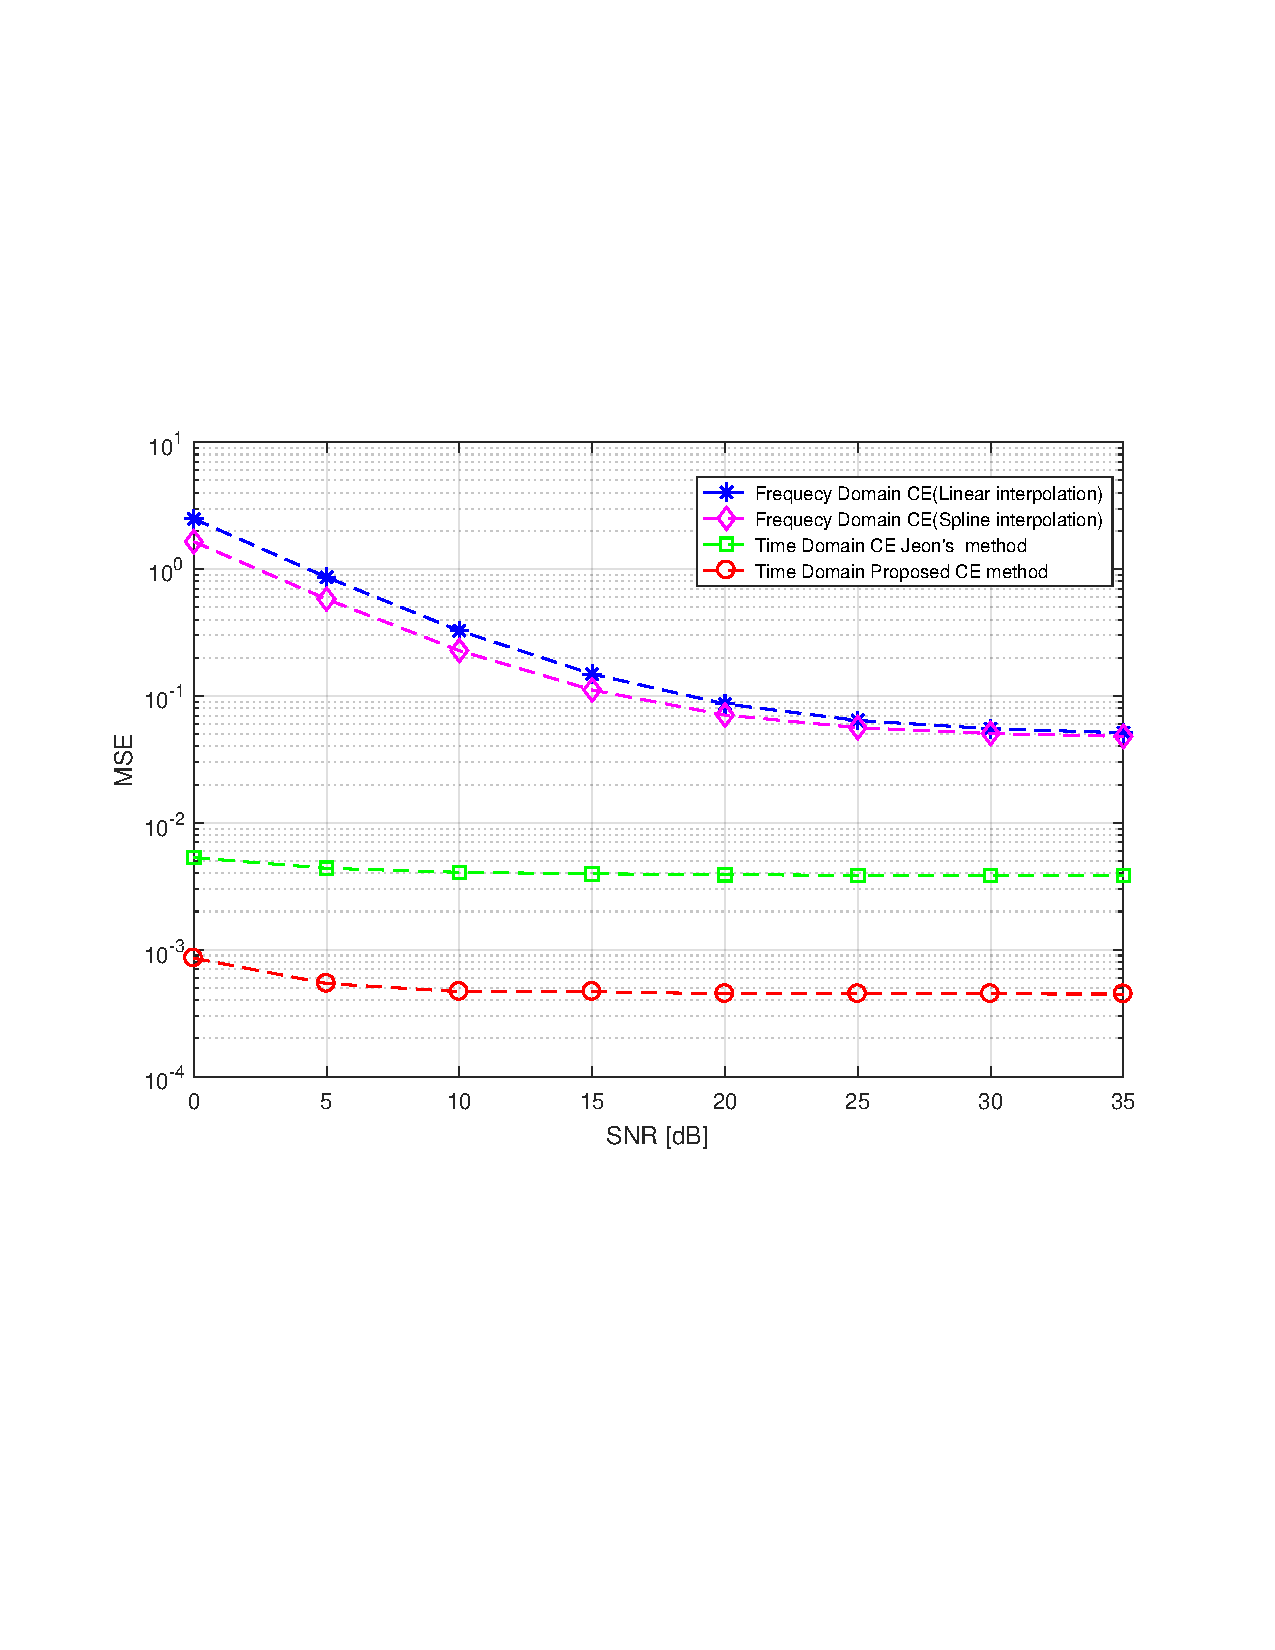
\includegraphics[width=1.0\linewidth]{figures/mse_1204Hz}
	\caption{Comparison of the MSE of the estimated channel obtained by the proposed	method with some standard methods for the channel with the Doppler frequency of $f_{d}=1204$Hz}
	\label{fig:1204hz}
\end{figure}
				
\begin{figure}
	\centering
	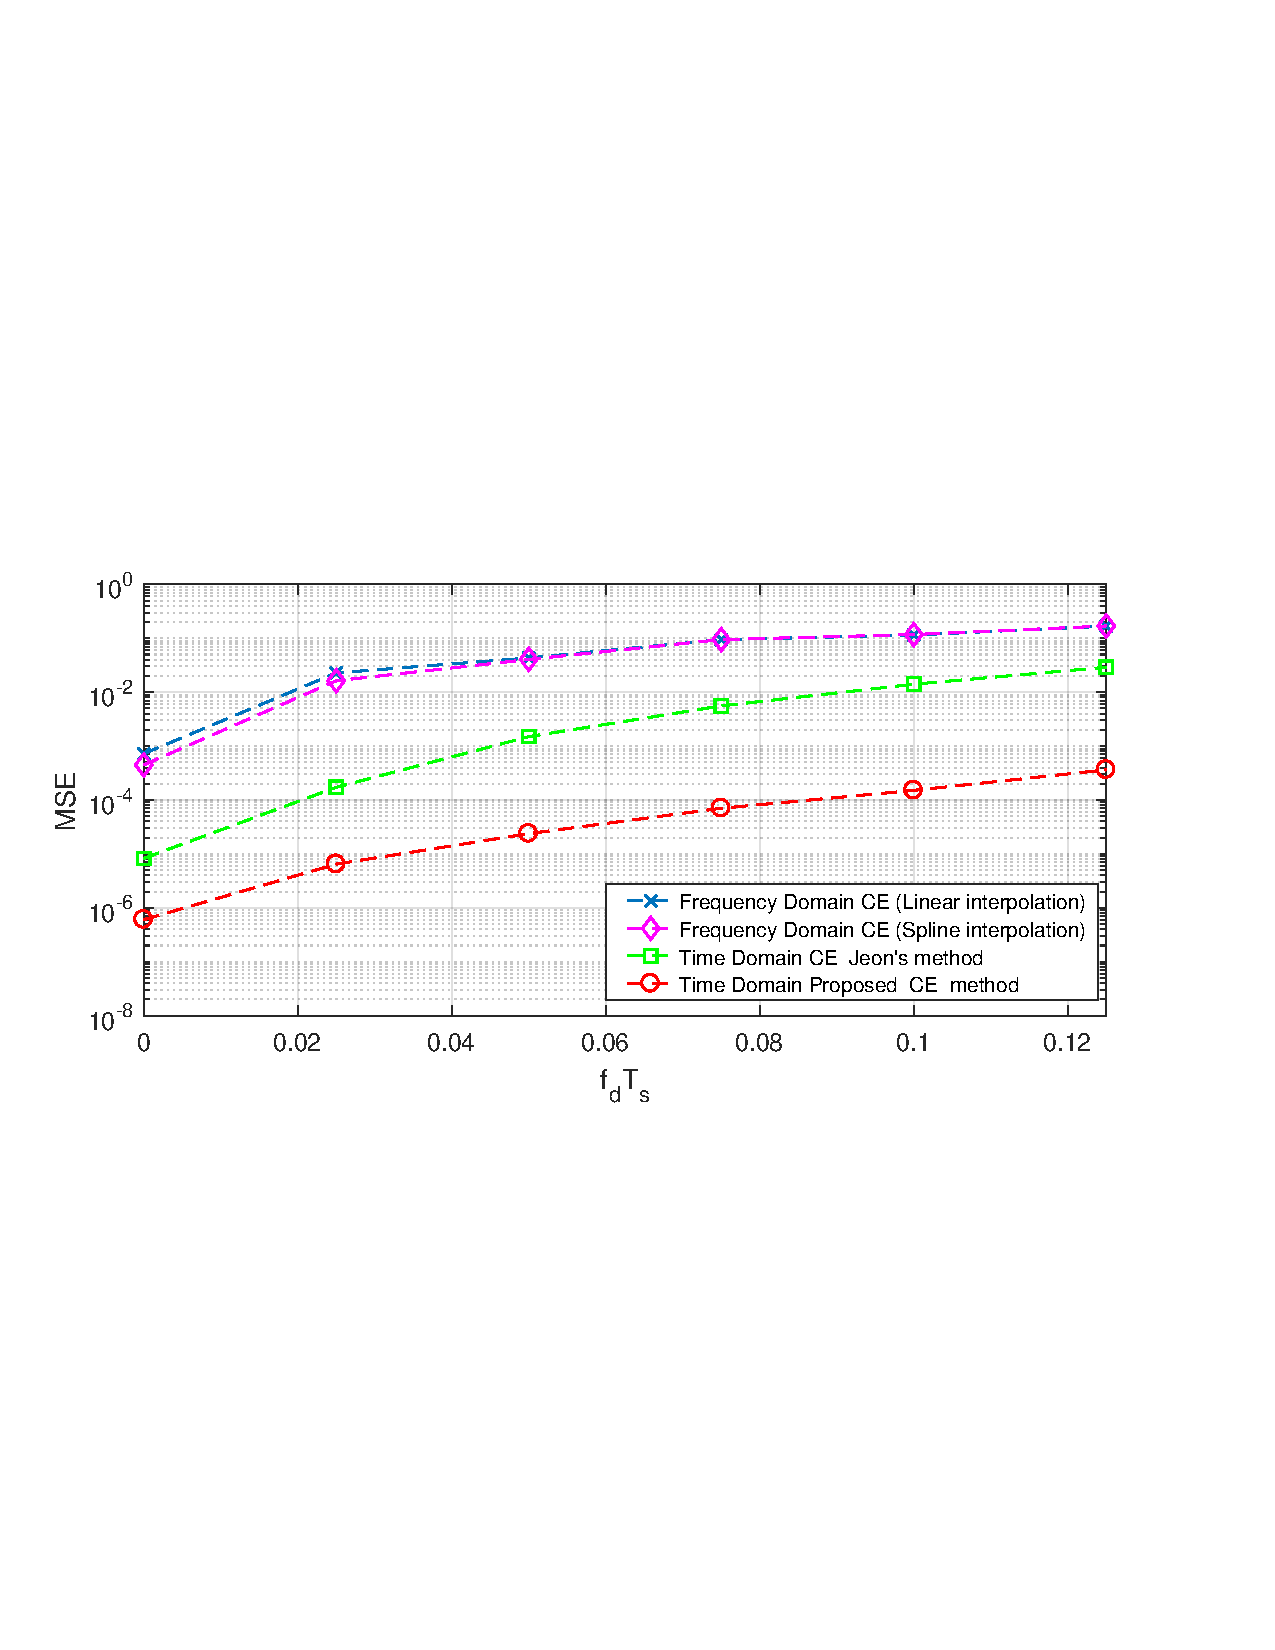
\includegraphics[width=1.0\linewidth]{figures/mse_speed.pdf}
	\caption{Comparison of the MSE of the estimated channel obtained by the proposed	method with some standard methods for the channel with the different speed}
	\label{fig:msespeed}
\end{figure}
				
\begin{figure}
	\centering
	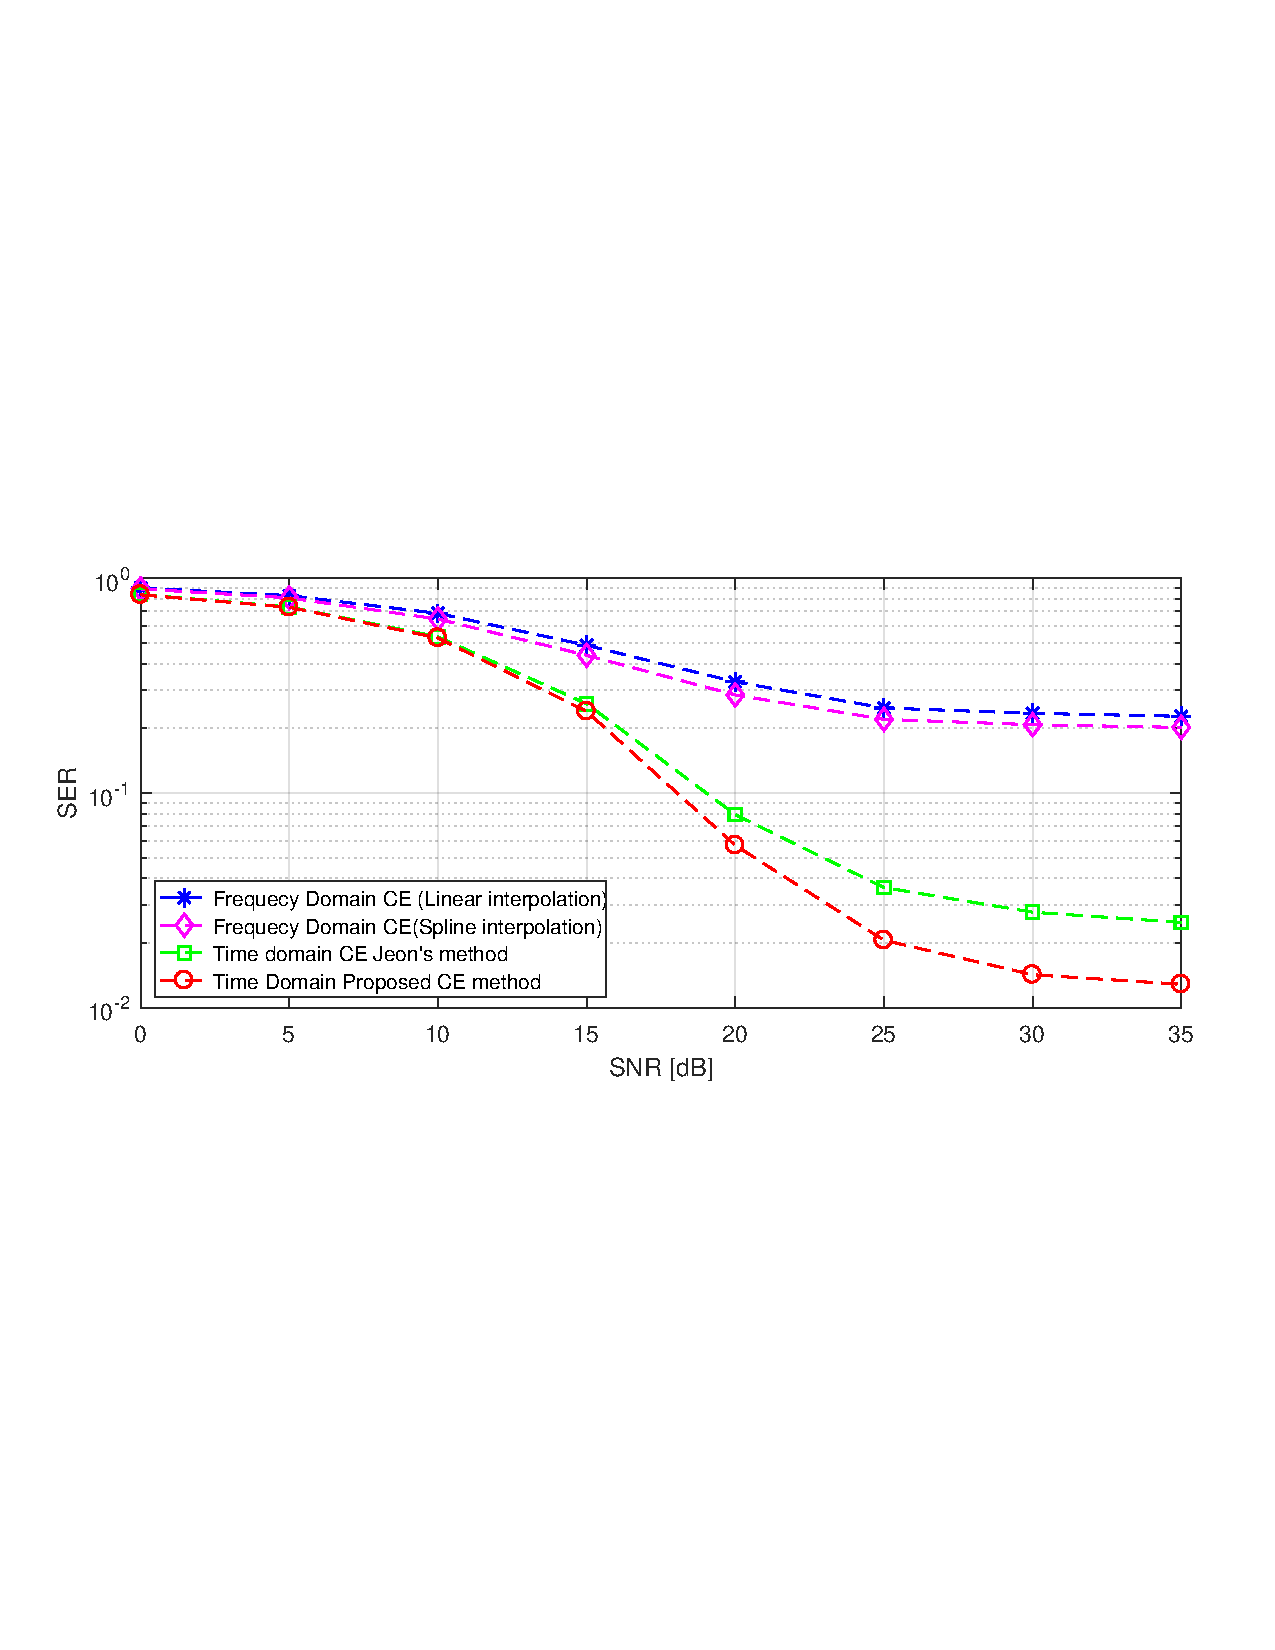
\includegraphics[width=1.0\linewidth]{figures/ser_722Hz.pdf}
	\caption{Comparison of the SER between the proposed
						method with some channel estimation methods with
						frequency of $f_{d}=722$Hz}
	\label{fig:ser722hz}
\end{figure}	
%	
\section{Conclusion}\label{section-5}
				
This paper proposed a time domain CE method using a special pilot symbol structure to protect the inserted pilot symbols from the multipath interference, and the Cubic Hermite interpolation technique to reconstruct the information of each sub-channel path in the time domain. The CIR can be therefore obtained from sampling interval to  sampling interval. Afterwards, the estimated CIR is applied to an ICI canceller to eliminate interference components introduced by the Doppler effect. The LTE-R channel and system parameters are taken into account for simulation setup. The simulation result show that our proposed method significantly outperform the state of the art methods. Thus, the proposed concept can be applied for OFDM systems over very fast time-varying channels, such as the LTE-R networks.
				
%\section*{Acknowledgement}
				
%This research was supported by a grant (17RTRP-B089546-04) from the Railway Technology Research %Project funded by the Ministry of Land, Infrastructure and Transport (MOLIT) of the Korean %government and by the Korea Agency for Infrastructure Technology Advancement (KAIA).			


%\bibliography{references}
\begin{thebibliography}{55}
	
\bib{Banerjee2016}{article}{
	author    = {Banerjee, Subharthi and Sharif, Hamid and others},
	title     = {A Survey of Wireless Communication Technologies \& Their Performance for High Speed Railways},
	journal   = {Journal of Transportation Technologies},
	year      = {2016},
	volume    = {6},
	number    = {01},
	pages     = {15},
}

\bib{Luo2012}{article}{
	author    = {Luo, Wantuan and Zhang, Ruiqiang and Fang, Xuming},
	title     = {A CoMP soft handover scheme for LTE systems in high speed railway},
	journal   = {EURASIP Journal on Wireless Communications and Networking},
	year      = {2012},
	volume    = {2012},
	number    = {1},
	pages     = {1--9},
}

\bib{Fokum2010}{article}{
	author    = {Fokum, Daniel T and Frost, Victor S},
	title     = {A survey on methods for broadband internet access on trains},
	journal   = {IEEE communications surveys \& tutorials},
	year      = {2010},
	volume    = {12},
	number    = {2},
	pages     = {171--185},
}  

\bib{Barhumi2005}{article}{
	author       = {Barhumi, Imad and Leus, Geert and Moonen, Marc},
	title        = {MMSE estimation of basis expansion models for rapidly time-varying channels},
	booktitle    = {Signal Processing Conference, 2005 13th European},
	year         = {2005},
	pages        = {1--5},
} 
\bib{Adireddy2002}{article}{
	author    = {Adireddy, Srihari and Tong, Lang and Viswanathan, Harish},
	title     = {Optimal placement of training for frequency-selective block-fading channels},
	journal   = {IEEE Transactions on Information Theory},
	year      = {2002},
	volume    = {48},
	number    = {8},
	pages     = {2338--2353},
}


\bib{Fan2014}{article}{
	author       = {Fan, Zhenkai and Lu, Zhaohua and Han, Yanjun},
	title        = {Accurate channel estimation based on Bayesian Compressive Sensing for next-generation wireless broadcasting systems},
	booktitle    = {Broadband Multimedia Systems and Broadcasting (BMSB), 2014 IEEE International Symposium on},
	year         = {2014},
	pages        = {1--5},
}


\bib{Mostofi2005}{article}{
	uthor    = {Mostofi, Yasamin and Cox, Donald C},
	title     = {ICI mitigation for pilot-aided OFDM mobile systems},
	journal   = {IEEE Transactions on Wireless Communications},
	year      = {2005},
	volume    = {4},
	number    = {2},
	pages     = {765--774},
}

\bib{Hijazi2009}{article}{
	author    = {Hijazi, Hussein and Ros, Laurent},
	title     = {Polynomial estimation of time-varying multipath gains with intercarrier interference mitigation in OFDM systems},
	journal   = {IEEE Transactions on Vehicular Technology},
	year      = {2009},
	volume    = {58},
	number    = {1},
	pages     = {140--151},
}


\bib{Simko2011}{article}{
	author       = {Simko, Michal and Mehlfuhrer, Christian and Zemen, Thomas and Rupp, Markus},
	title        = {Inter-carrier interference estimation in MIMO OFDM systems with arbitrary pilot structure},
	booktitle    = {Vehicular Technology Conference (VTC Spring), 2011 IEEE 73rd},
	year         = {2011},
	pages        = {1--5},
}


\bib{Edfors1998}{article}{
	author    = {Edfors, Ove and Sandell, Magnus and Van de Beek, J-J and Wilson, Sarah Kate and Borjesson, Per Ola},
	title     = {OFDM channel estimation by singular value decomposition},
	journal   = {IEEE Transactions on communications},
	year      = {1998},
	volume    = {46},
	number    = {7},
	pages     = {931--939},
}

\bib{Kaufman1983}{article}{
	author    = {Kaufman, Howard and Woods, J and Dravida, Subrahmanyam and Tekalp, A},
	title     = {Estimation and identification of two-dimensional images},
	journal   = {IEEE transactions on automatic control},
	year      = {1983},
	volume    = {28},
	number    = {7},
	pages     = {745--756},
}

\bib{Wang2016}{article}{
	author    = {Wang, Cheng-Xiang and Ghazal, Ammar and Ai, Bo and Liu, Yu and Fan, Pingzhi},
	title     = {Channel measurements and models for high-speed train communication systems: a survey},
	journal   = {IEEE Communications Surveys \& Tutorials},
	year      = {2016},
	volume    = {18},
	number    = {2},
	pages     = {974--987},
}

\bib{Guan2011}{article}{
	author       = {Guan, Ke and Zhong, Zhangdui and Ai, Bo},
	title        = {Assessment of LTE-R using high speed railway channel model},
	booktitle    = {Communications and Mobile Computing (CMC), 2011 Third International Conference on},
	year         = {2011},
	pages        = {461--464},
}

\bib{Matz2011}{article}{
	author  = {Matz, Gerald and Hlawatsch, Franz},
	title   = {Fundamentals of time-varying communication channels},
	journal = {Wireless Communications over Rapidly Time-Varying Channels, F. Hlawatsch and G. Matz, Eds. Academic Press},
	year    = {2011},
	pages   = {1--63},
}

\bib{Nguyen2004}{article}{
	author    = {Nguyen, VD and P{\"a}tzold, M},
	title     = {Least square channel estimation using special training sequences for MIMO-OFDM systems in the presence of intersymbol interference},
	booktitle = {Nordic Radio Symposium (NRS), Oulu, Finland},
	year      = {2004},
} 

\bib{Jeon1999}{article}{
	author    = {Jeon, Won Gi and Chang, Kyung Hi and Cho, Yong Soo},
	title     = {An equalization technique for orthogonal frequency-division multiplexing systems in time-variant multipath channels},
	journal   = {IEEE Transactions on Communications},
	year      = {1999},
	volume    = {47},
	number    = {1},
	pages     = {27--32},}
	
\bib{Cai2003}{article}{
	author    = {Cai, Xiaodong and Giannakis, Georgios B},
	title     = {Bounding performance and suppressing intercarrier interference in wireless mobile OFDM},
	journal   = {IEEE Transactions on Communications},
	year      = {2003},
	volume    = {51},
	number    = {12},
	pages     = {2047--2056},
}
	
\bib{Hsu2009}{article}{
	author    = {Hsu, Chao-Yuan and Wu, Wen-Rong},
	title     = {Low-complexity ICI mitigation methods for high-mobility SISO/MIMO-OFDM systems},
	journal   = {IEEE Transactions on vehicular technology},
	year      = {2009},
	volume    = {58},
	number    = {6},
	pages     = {2755--2768},
}

\bib{Liu2012}{article}{
	author    = {Liu, Guanghui and Zhidkov, Sergey V and Li, Hongliang and Zeng, Liaoyuan and Wang, Zhengning},
	title     = {Low-complexity iterative equalization for symbol-reconstruction-based OFDM receivers over doubly selective channels},
	journal   = {IEEE Transactions on Broadcasting},
	year      = {2012},
	volume    = {58},
	number    = {3},
	pages     = {390--400},
} 

\bib{Schniter2004}{article}{
	author    = {Schniter, Philip},
	title     = {Low-complexity equalization of OFDM in doubly selective channels},
	journal   = {IEEE Transactions on Signal processing},
	year      = {2004},
	volume    = {52},
	number    = {4},
	pages     = {1002--1011},
}

\bib{Fang2007}{article}{
	author    = {Fang, Kun and Leus, Geert},
	title     = {Low-complexity block turbo equalization for OFDM systems in time-and frequency-selective channels},
	booktitle = {The Third Annual IEEE BENELUX/DSP Valley Signal Processing Symposium},
	year      = {2007},
	pages     = {83--87},
}

\bib{Hu2003}{article}{
	author       = {Hu, Die and Yang, Luxi},
	title        = {Time-varying channel estimation based on pilot tones in OFDM systems},
	booktitle    = {Neural Networks and Signal Processing, 2003. Proceedings of the 2003 International Conference on},
	year         = {2003},
	volume       = {1},
	pages        = {700--703},
} 

\bib{Tang2007}{article}{
	author    = {Tang, Zijian and Cannizzaro, Rocco Claudio and Leus, Geert and Banelli, Paolo},
	title     = {Pilot-assisted time-varying channel estimation for OFDM systems},
	journal   = {IEEE Transactions on Signal Processing},
	year      = {2007},
	volume    = {55},
	number    = {5},
	pages     = {2226--2238},
}

\bib{Park2005}{article}{
	author    = {Park, Kyung Won and Cho, Yong Soo},
	title     = {An MIMO-OFDM technique for high-speed mobile channels},
	journal   = {IEEE Communications Letters},
	year      = {2005},
	volume    = {9},
	number    = {7},
	pages     = {604--606},
}
\bib{Cavers1991}{article}{
	author    = {Cavers, James K},
	title     = {An analysis of pilot symbol assisted modulation for Rayleigh fading channels (mobile radio)},
	journal   = {IEEE transactions on vehicular technology},
	year      = {1991},
	volume    = {40},
	number    = {4},
	pages     = {686--693},
}


\bib{Lau1994}{article}{
	author       = {Lau, HK and Cheung, SW},
	title        = {A pilot symbol-aided technique used for digital signals in multipath environments},
	booktitle    = {Communications, 1994. ICC'94, SUPERCOMM/ICC'94, Conference Record,'Serving Humanity Through Communications.'IEEE International Conference on},
	year         = {1994},
	pages        = {1126--1130},
}

\bib{Fritsch1980}{article}{
	author    = {Fritsch, Frederick N and Carlson, Ralph E},
	title     = {Monotone piecewise cubic interpolation},
	journal   = {SIAM Journal on Numerical Analysis},
	year      = {1980},
	volume    = {17},
	number    = {2},
	pages     = {238--246},
}

\bib{Qiu2010}{article}{
	author        = {Qiu, J and Tao, C and Liu, LIU},
	title         = {A novel OFDM channel estimation algorithm with ICI mitigation over fast fading channels},
	journal       = {Radioengineering},
	year          = {2010},
}

\bib{Luan2013}{article}{
	author    = {Luan, Fengyu and Zhang, Yan and Xiao, Limin and Zhou, Chunhui and Zhou, Shidong},
	title     = {Fading characteristics of wireless channel on high-speed railway in hilly terrain scenario},
	journal   = {International Journal of Antennas and Propagation},
	year      = {2013},
	volume    = {2013},
	publisher = {Hindawi Publishing Corporation},
}
	
\end{thebibliography}					
%\end{document}			
			
%\section*{Author Biography}			
%\begin{biography}{\includegraphics[width=66pt,height=86pt,draft]{blankfig}}{\textbf{Author Name.} This is sample author biography text this is sample author biography text this is sample author biography text this is sample author biography text this is sample author biography text this is sample author biography text this is sample author biography text this is sample author biography text this is sample author biography text this is sample author biography text this is sample author biography text this is sample author biography text this is sample author biography text this is sample author biography text this is sample author biography text this is sample author biography text this is sample author biography text this is sample author biography text this is sample author biography text this is sample author biography text this is sample author biography text.}
%\end{biography}
			
\end{document}
